% Reliability-horizon monitoring for world models.
% Drops into the official ICML style: place icml2025.sty next to this file and the
% \IfFileExists switch below will use it. Otherwise it compiles standalone as two-column
% article, so the manuscript is always buildable.
\documentclass[twocolumn,10pt]{article}

\usepackage{microtype}
\usepackage{graphicx}
\usepackage{booktabs}
\usepackage{amsmath,amssymb,amsfonts}
\usepackage{mathtools}
\usepackage{xcolor}
\usepackage[hidelinks]{hyperref}
\usepackage{url}
\usepackage{caption}
\usepackage{natbib}
\usepackage[margin=0.75in]{geometry}

\IfFileExists{icml2025.sty}{\usepackage[accepted]{icml2025}}{}

\captionsetup{font=small,labelfont=bf,skip=4pt}
\setlength{\tabcolsep}{4pt}
\renewcommand{\arraystretch}{1.06}

\newcommand{\Hstar}{H^{*}}
\newcommand{\Hhat}{\hat{H}}
\newcommand{\gphi}{g_{\phi}}
\newcommand{\rmse}{\mathrm{RMSE}}
\providecommand{\tabledir}{tables}

\title{Learning to Monitor the Reliability Horizon of Imagined Futures}
\author{Abhishek Rajdhar Dubey \\
  Independent Researcher \\
  \texttt{abhishekrajdhardubey@gmail.com}}
\date{}

\begin{document}
\twocolumn[
\maketitle
\begin{abstract}
\noindent
An agent that plans by imagining must decide how far to trust what it imagines. We study
whether a world model can learn a \emph{monitor} of that trust: a predictor of the
\emph{reliability horizon} $\Hstar$, the number of consecutive imagined steps whose predicted
state matches the environment exactly. In partially observed gridworlds, a learned monitor
predicts $\Hstar$ with Spearman $\rho = 0.573 \pm 0.011$ and improves on an
\emph{optimistically fitted} monotone single-scalar ceiling by $1.04$ MAE on average, with
per-seed bootstrap confidence intervals excluding zero. The monitor requires information from
the imagined rollout: restricted to time-$t$ features it fails to beat that ceiling on any
seed. Under distribution shift the monitor fails \emph{anti-conservatively}, predicting
horizons near $20$ where the true horizon is $4$--$8$; it is most confident where the world
model is least reliable. Two repairs we tested, rank-normalising the monitor's inputs and
gating on latent novelty, do not recover it: the uncertainty signals retain aggregate
separation between distributions while losing within-distribution rank-informativeness.
Refitting the monitor with a single shifted configuration in its training set moves a
never-seen configuration from MAE $16.77$ / $\rho\,0.135$ to MAE $3.58$ / $\rho\,0.766$, and a
size-matched control indicates this is not explained by sample count alone. The restoration is
selective: shifts that alter geometry transfer strongly to other geometric shifts
($\rho\,0.73$--$0.86$) but weakly to noise-driven ones ($\rho \approx 0.31$). The core result
also appears in a world model with no recurrence and no autoregressive latent feedback, though
monitors transfer only partially across architectures. These results suggest that
simulation-based reliability monitoring is measurable and not architecture-specific, but that
its calibration is learned from the distribution of failures the world model has experienced
rather than being an invariant property of uncertainty.
\end{abstract}
\vspace{0.28in}
]

\section{Introduction}
\label{sec:intro}

World models are used to plan by imagining: an agent rolls its learned dynamics forward under
candidate actions and acts on the result \citep{ha2018world,hafner2019planet,hafner2020dream}.
The question usually asked of such a model is whether it predicts the future accurately. The
question an acting agent actually needs answered is different and sharper: \emph{for how many
steps does this particular imagined rollout remain worth acting on?} Too short a horizon wastes
the model; too long, and the agent plans against a hallucination.

The standard answer thresholds an uncertainty signal --- roll forward, stop when ensemble
disagreement or predictive entropy crosses a bound \citep{janner2019mbpo,chua2018pets}. That
recipe rests on a premise which prior work supports: uncertainty correlates with realised
rollout error. We call this \textbf{Claim~A}. It licenses ranking states by riskiness, and
nothing more.

We study a stronger statement. \textbf{Claim~B}: an agent can learn a \emph{monitor} that
predicts the horizon itself, per state, as a quantity. The distinction matters because a
threshold rule is only ever as good as the monotone map from uncertainty to trust. If that map
exhausts the available signal, then nothing beyond Claim~A has been demonstrated, however
elaborate the machinery.

Our central methodological device is therefore a control rather than a baseline. For each
uncertainty scalar we fit an isotonic regression from that scalar to $\Hstar$ \emph{on the
evaluation data itself}. This is deliberately optimistic --- it is the best attainable
performance of \emph{any} monotone function of that signal, with no generalisation gap.
Beating it is the minimum evidence that Claim~B says something Claim~A does not.

Having established that the monitor works in distribution, we ask when it stops working,
whether simple corrections recover it, and what kind of experience does. The negative results
carry most of the content: our aim is a characterisation of when simulation-based reliability
monitoring works and fails, not a new uncertainty metric.

\paragraph{Contributions.}
\begin{enumerate}\itemsep1pt
\item An operational notion of the imagined reliability horizon with an exactly checkable
target, and evidence that a learned rollout monitor predicts it beyond an optimistic
single-scalar uncertainty ceiling (\S\ref{sec:core}).
\item Evidence that information from the imagined rollout is necessary: a monitor restricted
to time-$t$ features does not beat that ceiling on any seed (\S\ref{sec:rollout}).
\item A failure mode under distribution shift in which the monitor becomes
\emph{anti-conservative}, which we trace to loss of feature rank-informativeness rather than of
scale (\S\ref{sec:ood}, \S\ref{sec:mech}).
\item Evidence that exposure to a shifted distribution can substantially restore transfer, that
the effect is not explained by sample count alone, and that it is selective across shift types
and across world-model architectures (\S\ref{sec:exposure}--\S\ref{sec:asym}).
\end{enumerate}

\section{Related Work}
\label{sec:related}

\paragraph{World models and latent imagination.}
Latent dynamics models trained from pixels or symbols underpin modern model-based control
\citep{ha2018world,hafner2019planet,hafner2020dream,hafner2021dreamerv2,hafner2023dreamerv3}.
We adopt the same recurrent state-space structure, but our object of study is not control
performance; it is the horizon over which the imagined rollout is exact.

\paragraph{Uncertainty in learned dynamics.}
Deep ensembles and their disagreement are the standard epistemic signal
\citep{lakshminarayanan2017ensembles,chua2018pets}, alongside dropout- and
distribution-based estimates \citep{gal2016dropout,kendall2017uncertainties}. Recent work
propagates epistemic uncertainty through long autoregressive rollouts and uses it to make
offline model-based RL work on physical robots \citep{li2025uncertainty}. These establish
Claim~A. We treat the best monotone map from such a scalar to the horizon as a control to be
beaten, not as a method to be improved.

\paragraph{Adaptive rollout length.}
Model-based RL truncates imagined rollouts when uncertainty exceeds a threshold
\citep{janner2019mbpo}, and rollout length can be tuned online by treating it as a meta-level
decision problem \citep{bhatia2022adaptive}. These are \emph{online} rules that observe the
rollout, or the training run, as it unfolds; we include threshold truncation as a baseline.
Related adaptive machinery appears in latent visual MPC: ELVIS gates a time-varying
$\lambda$ --- trading bootstrapping against look-ahead --- using an upper-confidence-bound
score from an ensemble of latent critics \citep{du2026elvis}. That adapts the \emph{value
estimator}, not a predicted horizon. Our monitor differs from all of these in predicting a
horizon as a quantity and being evaluated against ground truth rather than by downstream
return.

\paragraph{Horizon certificates.}
Two recent works certify how long a learned model can be trusted. \citet{wang2026certified}
derives predictability certificates for equivariant latent world models from the finite-time
Lyapunov spectrum, with expanding channels giving logarithmic horizons and contracting channels
bounded error floors. \citet{wang2026conformal} calibrates trust-horizon curves by split
conformal prediction and transports them across a symmetry orbit, reporting a median
certified-to-measured horizon ratio of $0.67$ and zero anti-conservative violations across
their stable audits. Both require known group symmetry and produce certificates that are
orbit-level and worst-case; ours is a learned per-state estimate with no symmetry assumption
and, notably, \emph{no} such conservatism guarantee --- the anti-conservative failure we
document in \S\ref{sec:ood} is precisely what a conformal construction is designed to exclude.

\paragraph{Self-estimated rollout error.}
\citet{scheinker2026roundtrip} trains a bidirectional latent diffusion model and uses the
discrepancy of a forward-then-backward rollout as a self-supervised proxy for rollout error,
reporting Spearman correlations of $0.91$--$0.98$ against realised error on
magnetohydrodynamics, astrophysical mixing layers and face video. That method requires a model
trained to run in both directions and an extra backward pass, and its domains contain no
acting agent; our \S\ref{sec:rollout} result --- that a forward rollout is necessary --- puts
us on the same side of the a-priori boundary, at lower cost and without invertibility.
\citet{song2026rollout} instead explains rollout error post hoc in graph world models, splitting
long-horizon error into a topology factor governed by the graph spectral radius and a model
factor; that analysis is model-level rather than per-state.

\paragraph{Failure prediction and data coverage.}
\citet{berger2026biased} report a negative result closely related to ours: in Dreamer-style
RSSM latent rollouts, ensemble disagreement captures local epistemic uncertainty but does not
reflect error accumulated over long rollouts, because rollouts are pulled toward well-modelled
attractor regions where uncertainty declines even as deviation grows. \citet{hansen2026hallucination} argue that hallucination in large visual world models is predictable from
coverage-related signals and preventable by coverage-aware data collection, concluding it is
``inherently a data coverage issue''. Our \S\ref{sec:exposure} result is convergent evidence
from a different direction: what fails under shift is repaired by exposure to the right kind of
failure, not by better use of the uncertainty signal already available.

\paragraph{Calibration, selective prediction, and shift.}
Calibration of modern networks \citep{guo2017calibration}, selective prediction with a reject
option \citep{geifman2017selective}, and distribution-free coverage via conformal methods
\citep{angelopoulos2021conformal} all target when a prediction should be trusted. Our setting
differs in that the quantity to be trusted is a \emph{depth} rather than a label, and in that
the failure we document is a loss of ranking rather than of coverage. That uncertainty
estimates degrade under shift is well documented \citep{ovadia2019trust,hendrycks2017baseline};
we add that the degradation here inverts the safety-relevant direction.

\paragraph{Positioning.} To our knowledge the combination we study --- a learned, per-state
horizon monitor, evaluated against an optimistic monotone control, and characterised across
distribution shifts and world-model architectures --- has not been reported.

\section{Problem Formulation}
\label{sec:problem}

\paragraph{Setting.}
An agent observes $o_t$ and acts with $a_t$. A world model with parameters $\theta$ maintains a
belief $(h_t, z_t)$ and predicts forward without further observations. Given an action sequence
$a_{t:t+H-1}$ known at planning time, the model produces an \emph{imagined rollout}
\begin{equation}
\begin{aligned}
\hat{\tau}_{t:t+H} &= \big(\hat{s}_{t+1}, \hat{s}_{t+2}, \dots, \hat{s}_{t+H}\big), \\
\hat{s}_{t+k} &= \mathrm{dec}_\theta(h_{t+k}, z_{t+k}).
\end{aligned}
\end{equation}

\paragraph{Reliability horizon.}
With $E_H = d(\hat{s}_{t+H}, s_{t+H})$ the discrepancy against the realised state and a
tolerance $\varepsilon$, we define
\begin{equation}
\Hstar(s_t) \;=\; \max\big\{\, H \le H_{\max} \;:\; E_h < \varepsilon \ \ \forall\, h \in 1..H \,\big\}.
\label{eq:hstar}
\end{equation}
Equation~\eqref{eq:hstar} is a \emph{first-failure} definition: once imagination diverges it is
operationally unusable even if it later re-synchronises by coincidence. We set
$H_{\max} = 30$.

\paragraph{Instantiation.}
Observations are $5\times5$ egocentric symbolic views, so grid size never enters the
observation. The model predicts size-agnostic state \emph{factors} --- direction $\mathrm{dir}$,
a binary $\mathrm{moved}$ indicating whether the transition changed the agent's cell, plus
carrying and door state --- and position is reconstructed by integration,
\begin{equation}
\hat{p}_{t+H} - p_t \;=\; \sum_{k=1}^{H} \mathrm{moved}_{t+k}\cdot u(\mathrm{dir}_{t+k-1}),
\label{eq:integrate}
\end{equation}
with $u(\cdot)$ the unit vector of a direction. $E_H$ is the Manhattan error of
\eqref{eq:integrate} and $\varepsilon = 1$, so $E_H < \varepsilon$ means the model places the
agent in \emph{exactly} the correct cell. We verify \eqref{eq:integrate} exactly on the true
factors for every configuration before modelling.

This makes the object of study concrete. The load-bearing factor is $\mathrm{moved}$ --- whether
the cell ahead is free --- which is precisely what partial observability hides. Imagination
stays exact roughly as long as the planned path remains inside the region the agent has already
seen.

\paragraph{The monitor.}
Let $x_t$ be a feature vector computed at time $t$, grouped as: \emph{a-priori} features
(belief state, one-step uncertainty, statistics of the current observation), \emph{rollout}
features (per-step ensemble disagreement, predictive entropy, spread of imagined displacement
across ensemble members), and \emph{action} features (the planned sequence). The monitor
\begin{equation}
\Hhat_t = \gphi(x_t), \qquad \gphi: x_t \mapsto \Delta^{H_{\max}+1}
\end{equation}
outputs a distribution over $\Hstar \in \{0,\dots,H_{\max}\}$, giving both a point estimate
(its mean) and $P(\Hstar \ge h)$ for calibration. Crucially, $x_t$ may not depend on any
observation, state, or error at time $>t$; we verify this by corrupting every future field and
checking that all features are bit-identical while $\Hstar$ changes.

\paragraph{The Claim-A ceiling.}
For a scalar uncertainty signal $u$, let $\mathcal{M}$ be the set of monotone maps
$\mathbb{R}\to\mathbb{R}$. The ceiling is
\begin{equation}
C_A(u) \;=\; \min_{m \in \mathcal{M}} \ \frac{1}{N}\sum_{i=1}^{N} \big| m(u_i) - \Hstar_i \big|,
\label{eq:ceiling}
\end{equation}
computed by isotonic regression \emph{fitted on the evaluation split}. It therefore has no
generalisation gap and is optimistic by construction; we report the minimum of
\eqref{eq:ceiling} over all candidate scalars. A monitor that beats it uses structure that no
monotone function of any single uncertainty scalar can express.

\section{World Models and Architectures}
\label{sec:wm}

We train three world models that share data, seeds, targets and all downstream code, differing
only in dynamics (Figure~\ref{fig:arch}b, Table~\ref{tab:arch}). M1 and M2 are GRU-based
recurrent state-space models of different capacity. M3 replaces recurrence with causal
self-attention and has \emph{no autoregressive latent feedback}: observations are replaced by a
learned mask token wherever unavailable, so imagination is a single masked forward pass rather
than a rolled-forward prior. M3 exposes the same interface and produces the same head set, so
$\Hstar$, the features, and every downstream computation are identical across architectures.

\begin{figure*}[t]
\centering
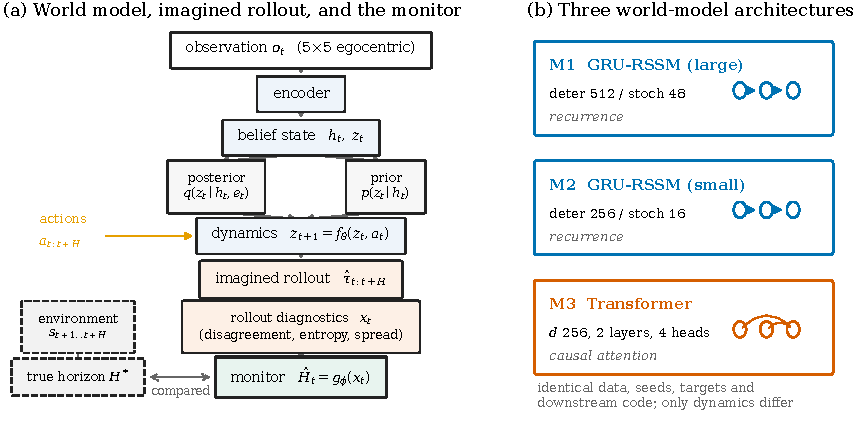
\includegraphics[width=\textwidth]{figures/architecture.pdf}
\caption{\textbf{(a)} The world model produces an imagined rollout from a belief state and a
planned action sequence; rollout diagnostics $x_t$ feed the monitor $\gphi$, whose output
$\Hhat_t$ is compared against the reliability horizon $\Hstar$ measured against the
environment (dashed path, available only at evaluation time). \textbf{(b)} The three
architectures. M1/M2 propagate a recurrent state; M3 aggregates history by causal attention and
has no autoregressive latent feedback.}
\label{fig:arch}
\end{figure*}

\begin{table*}[t]
\centering\small
\begin{tabular}{llllcccc}
\toprule
& architecture & dynamics & size & $H^*$ on A & MAE $\downarrow$ & $\rho$ $\uparrow$ & vs.\ ceiling \\
\midrule
M1 & GRU-RSSM (large) & gated recurrence & deter 512, stoch 48 & 15.59 & 6.408 & +0.584 & $+1.355$ \\
M2 & GRU-RSSM (small) & gated recurrence & deter 256, stoch 16 & 13.65 & 6.351 & +0.551 & $+1.050$ \\
M3 & Transformer & causal attention & $d$ 256, 2 layers, 4 heads & 16.58 & 6.432 & +0.513 & $+0.993$ \\
\bottomrule
\end{tabular}
\caption{World-model architectures, with in-distribution monitor performance and the margin
over that architecture's own Claim-A ceiling. Single seed, $K=3$ ensemble members.}
\label{tab:arch}
\end{table*}

\section{Experimental Setup}
\label{sec:setup}

\paragraph{Configurations.}
A (\texttt{DoorKey-16x16}) is the training distribution. Shifts: B (\texttt{FourRooms},
unseen layout topology), C (A with $15\%$ action slip), D (\texttt{MultiRoom-N6}, long
corridors), E (\texttt{SimpleCrossingS11N5}, unseen maze family), F2 (observation noise), F3
($20\%$ action dropout). World models and monitors are fitted on A unless stated.

\paragraph{Protocol.}
All decision rules were frozen before the corresponding evaluation across five
pre-registration documents; departures are logged with timing. Layout seeds are disjoint across
world-model training, monitor training, validation and test, and the monitor trains on episodes
the world model never saw, so $\Hstar$ is not inflated by memorisation. Model selection uses
validation only. We use three training seeds with $K=5$ ensemble members, and report
episode-clustered bootstrap intervals over $2000$ resamples.

\paragraph{Two measurement details that affect comparisons.}
First, $21\%$ of A-test targets sit at the ceiling $H_{\max}=30$ and are therefore
right-censored; MAE is inflated and the upper tail is unidentified. Second, the main run
evaluates shifts on the \emph{full} configuration split, whereas the transfer experiments
(\S\ref{sec:exposure}--\S\ref{sec:asym}) partition each shifted configuration $60/20/20$ by
episode and evaluate only on the held-out $20\%$. Baselines therefore differ slightly between
sections --- for example the no-exposure monitor reaches $\rho = 0.165$ on D in
Table~\ref{tab:ood} and $\rho = 0.135$ on D's test portion in Table~\ref{tab:transfer} --- and
numbers should be compared within a table, not across.

\paragraph{Hypothesis ledger.}
Table~\ref{tab:ledger} lists all nine pre-registered hypotheses with their frozen verdicts.
Five were not supported. We report them in the main text rather than the appendix.

\begin{table*}[t]
\centering\footnotesize
\resizebox{\textwidth}{!}{\begin{tabular}{llllp{3.3cm}}
\toprule
& question & protocol & verdict & note \\
\midrule
H1 & Uncertainty correlates with future error & main run & Supported & weak; the premise, not the result \\
H2 & Monitor beats best monotone single-scalar map & main run, 3 seeds & \textbf{Supported} & $+1.04$ MAE, CIs exclude 0 \\
H2$'$ & Same, without imagined-rollout features & main run, 3 seeds & Not supported & rollout information is necessary \\
H3 & Horizon drops before failure under shift & main run, 3 seeds & Not supported & fails anti-conservatively \\
H4 & Adaptive horizon improves planning at lower compute & 60 paired episodes & Not supported & \emph{weak test}: monotone frontier \\
H5 & OOD failure repaired by rank-norm / novelty gate & 3 seeds, 4 arms & Not supported & rank-informativeness, not scale \\
H6 & Shift exposure restores transfer & 3 seeds + size-matched & \textbf{Supported} & $\rho$ 0.135 $\to$ 0.766 on unseen D \\
H7 & Phenomenon is architecture-general & 3 architectures, 1 seed & Supported (H2); partial (H6) & monitor only partly portable \\
H8 & Shift-type taxonomy predicts transfer & 3 seeds, 2 new configs & Not supported & geometric half confirmed; F invalid \\
H9 & Noise-driven shifts transfer to each other & 3 seeds, validity gate & Not supported & 0.444 vs 0.50 bar; taxonomy withdrawn \\
\bottomrule
\end{tabular}}
\caption{All pre-registered hypotheses and their frozen verdicts. H4 is labelled a weak test
because the planning task's compute--performance frontier turned out to be monotone, leaving no
interior optimum for an adaptive horizon to find. H8/H9 withdrew a proposed shift-type
taxonomy; \S\ref{sec:asym} reports the asymmetry the data support instead.}
\label{tab:ledger}
\end{table*}

\section{Results}

\subsection{The monitor predicts the horizon}
\label{sec:core}

On A-test, $\Hstar$ has mean $15.60$ and interquartile range $20$--$21$, so the target is not
degenerate. Table~\ref{tab:main} reports the comparison and Figure~\ref{fig:main} shows it
per state.

The monitor attains MAE $6.416 \pm 0.087$ and $\rho = 0.573 \pm 0.011$ (mean $\pm$ s.d.\ over
three seeds; the feature-group variant selected on validation differed by seed, so we also
report fixed variants). Against the optimistic ceiling of \eqref{eq:ceiling} it improves by
$1.080$, $1.102$ and $0.936$ MAE on the three seeds, with paired bootstrap lower bounds
$0.978$, $1.010$ and $0.854$ --- all excluding zero. Against a constant predictor it improves
by $2.51$--$2.63$ MAE. In distribution the predictive distribution is well calibrated, with
expected calibration error $0.023$--$0.041$ for $P(\Hstar \ge h)$, $h \in \{3,5,10,20\}$.

Two comparisons sharpen the result. The monitor beats \emph{online truncation} --- stopping the
rollout when imagined displacement spread exceeds one cell --- by $1.99$ MAE. And a
\emph{privileged} predictor given the true local $11\times11$ grid together with the ordered
action sequence performs \emph{worse} ($\rho = 0.226$) than the monitor. Knowing the
environment is not sufficient; what the monitor exploits is the model's relationship to it.

\begin{figure}[t]
\centering
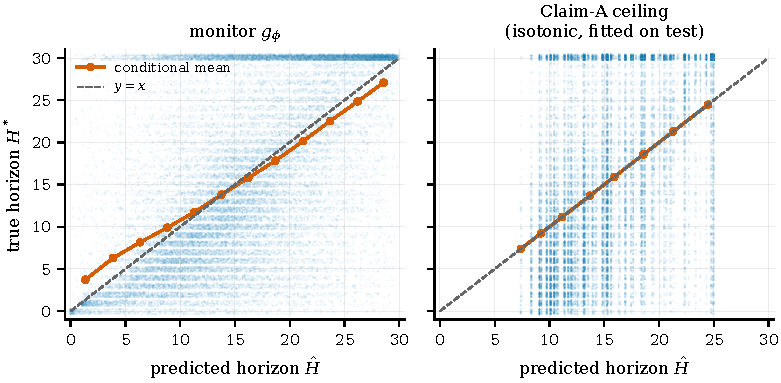
\includegraphics[width=\columnwidth]{figures/main_result.pdf}
\caption{Predicted versus true reliability horizon, pooled over three seeds
($3\times11{,}100$ states). Orange: conditional mean in bins of the prediction. The optimistic
ceiling (right) compresses its predictions into a narrow band and cannot express the extremes
of the target.}
\label{fig:main}
\end{figure}

\begin{table}[t]
\centering\footnotesize
\resizebox{\columnwidth}{!}{\begin{tabular}{lccc}
\toprule
method & MAE $\downarrow$ & Spearman $\rho$ $\uparrow$ & $R^2$ $\uparrow$ \\
\midrule
\textbf{Monitor $g_\phi$} (per-seed selected) & \textbf{6.416}\,$\pm$\,0.087 & \textbf{0.573}\,$\pm$\,0.011 & \textbf{0.318} \\
\quad \texttt{no\_latent} & 6.394\,$\pm$\,0.068 & 0.580\,$\pm$\,0.005 & 0.331 \\
\quad \texttt{full} & 6.457\,$\pm$\,0.080 & 0.566\,$\pm$\,0.005 & 0.304 \\
\quad uncertainty only & 6.604\,$\pm$\,0.109 & 0.553\,$\pm$\,0.012 & 0.301 \\
\midrule
Claim-A ceiling (isotonic, on test) & 7.456\,$\pm$\,0.158 & 0.459 & 0.224 \\
Strict a-priori (no rollout) & 8.065\,$\pm$\,0.087 & 0.372\,$\pm$\,0.003 & 0.119 \\
Hand-crafted + actions & 8.274\,$\pm$\,0.095 & 0.320\,$\pm$\,0.005 & 0.107 \\
Online truncation & 8.384\,$\pm$\,0.082 & 0.298\,$\pm$\,0.011 & 0.096 \\
Privileged: true local grid & 8.628\,$\pm$\,0.067 & 0.226\,$\pm$\,0.006 & 0.030 \\
Fixed horizon (median of val) & 8.975\,$\pm$\,0.101 & 0.000\,$\pm$\,0.000 & -0.010 \\
Random horizon & 11.002\,$\pm$\,0.047 & 0.001\,$\pm$\,0.004 & -0.721 \\
\bottomrule
\end{tabular}}
\caption{In-distribution horizon prediction on A-test, mean $\pm$ s.d.\ over three seeds. The
Claim-A ceiling is fitted on the evaluation split and is therefore optimistic. Bold marks the
primary monitor only.}
\label{tab:main}
\end{table}

\subsection{Rollout information is necessary}
\label{sec:rollout}

Restricting $\gphi$ to strictly time-$t$ features --- belief state, one-step uncertainty,
planned actions, statistics of the current observation, and no quantity computed from the
imagined rollout --- costs the effect entirely: MAE $8.065 \pm 0.087$, which is \emph{worse}
than the ceiling by $0.464$, $0.630$ and $0.735$ on the three seeds. The signal the monitor
exploits lives in the internal disagreement of the imagined trajectory. The honest reading of
``before observing the future'' is therefore: before observing it, but after imagining it.

\subsection{Under shift the monitor fails anti-conservatively}
\label{sec:ood}

Table~\ref{tab:ood} and Figure~\ref{fig:ood} report the shift results. In distribution the
monitor is nearly unbiased. Under shift the true horizon collapses to $4$--$8$ while the
prediction \emph{rises} to $13$--$21$, and the ranking quality falls from $\rho = 0.573$ to
$0.165$--$0.271$.

The direction matters. A monitor that degraded to noise would be useless; one that becomes
\emph{more} confident exactly where the world model is least reliable is worse than useless for
any application that would gate imagination on it.

\begin{figure}[t]
\centering
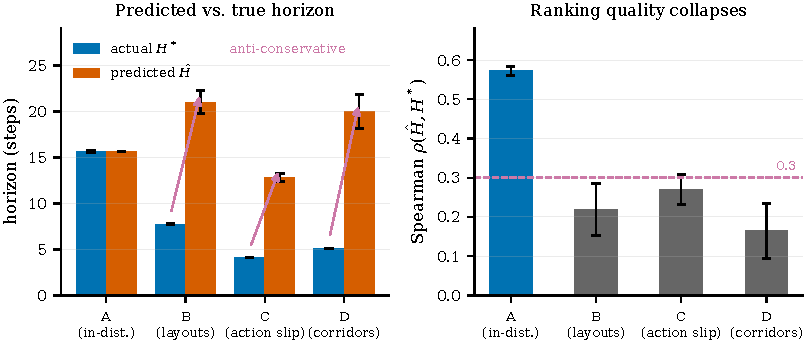
\includegraphics[width=\columnwidth]{figures/ood_failure.pdf}
\caption{Left: true and predicted horizon by configuration; the gap opens in the unsafe
direction under shift. Right: ranking quality against the $0.3$ reference used in the frozen
decision rules. Bars are means over three seeds, error bars s.d.}
\label{fig:ood}
\end{figure}

\begin{table}[t]
\centering\footnotesize
\begin{tabular}{lccc}
\toprule
configuration & true $H^*$ & predicted $\hat H$ & Spearman $\rho$ \\
\midrule
A (in distribution) & 15.60 & 15.67 & +0.573 \\
\midrule
B (unseen layouts) & 7.75 & \textbf{21.01} & +0.219 \\
C (action slip) & 4.11 & \textbf{12.82} & +0.271 \\
D (long corridors) & 5.11 & \textbf{19.97} & +0.165 \\
\midrule
\multicolumn{4}{l}{\emph{Repair attempts (H5), predicted $\hat H$ on each split}}\\
\quad no repair & \multicolumn{3}{c}{B 21.56\quad C 13.59\quad D 21.15} \\
\quad rank-normalised inputs & \multicolumn{3}{c}{B 20.99\quad C 16.08\quad D 21.29} \\
\quad novelty gate & \multicolumn{3}{c}{B 20.25\quad C 13.12\quad D 19.95} \\
\quad both & \multicolumn{3}{c}{B 19.78\quad C 15.56\quad D 20.12} \\
\bottomrule
\end{tabular}
\caption{Distribution-shift failure and the two repair attempts. Predicted horizons rise where
true horizons fall. Neither repair restores conservatism. Evaluated on full configuration
splits.}
\label{tab:ood}
\end{table}

\subsection{Simple repairs do not recover it}
\label{sec:repair}

We tested two corrections, neither fitted on shifted data: replacing each uncertainty feature
by its within-split quantile rank, and multiplying the prediction by a novelty gate
$\exp(-\lambda \max(0, \nu - \tau))$ whose constants are set on in-distribution validation so
that the gate is inert in distribution. Both fail on all three seeds
(Table~\ref{tab:ood}); predictions remain near $20$ against true horizons of $4$--$8$, and
rank-normalisation makes configuration C worse. \S\ref{sec:mech} explains why.

\subsection{Exposure to a shifted distribution restores transfer}
\label{sec:exposure}

We refit $\gphi$ on combinations of configurations, retraining no world model. Each shifted
configuration is partitioned $60/20/20$ by episode with the test portion evaluation-only in
every regime, so ``seen'' and ``unseen'' cells are directly comparable
(Table~\ref{tab:transfer}, Figure~\ref{fig:transfer}).

On D, never seen in training, the regime $\mathrm{A{+}B{+}C}$ moves MAE from $16.768$ to
$3.584$ and $\rho$ from $0.135$ to $0.766$, and the prediction becomes appropriately
conservative. A size-matched control, subsampling every regime to the A-only anchor count,
reproduces the effect (MAE $3.622$, $\rho = 0.762$). We therefore conclude that the effect is
\emph{not explained by sample count alone}; we do not claim that diversity is its only cause.
Adding a second shift changes little ($\mathrm{A{+}B}\to$D gives $\rho = 0.771$), so within
this environment family the marginal value of further shifts was small.

\begin{figure}[t]
\centering
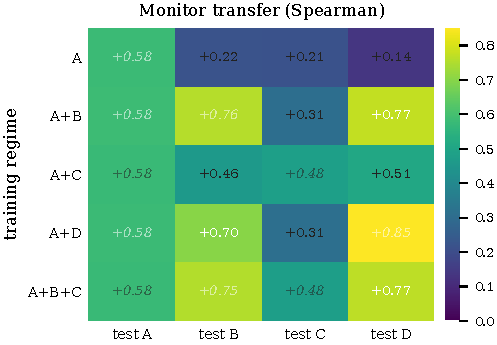
\includegraphics[width=\columnwidth]{figures/transfer_heatmap.pdf}
\caption{Monitor transfer. Rows are training regimes, columns held-out configurations; italic
cells denote a configuration seen during monitor training. Exposure to one shift lifts
performance on configurations never seen.}
\label{fig:transfer}
\end{figure}

\begin{table}[t]
\centering\small
\begin{tabular}{lcccc}
\toprule
training regime & test A & test B & test C & test D \\
\midrule
A & \emph{+0.580} & +0.218 & +0.213 & +0.135 \\
A+B & \emph{+0.584} & \emph{+0.755} & +0.306 & +0.771 \\
A+C & \emph{+0.576} & +0.461 & \emph{+0.479} & +0.510 \\
A+D & \emph{+0.580} & +0.699 & +0.311 & \emph{+0.847} \\
A+B+C & \emph{+0.577} & \emph{+0.754} & \emph{+0.477} & +0.766 \\
\bottomrule
\end{tabular}
\caption{Spearman $\rho$ by training regime, mean over three seeds. Italic entries are
configurations seen in training. Evaluated on $20\%$ held-out portions.}
\label{tab:transfer}
\end{table}

\subsection{Architecture generality and monitor portability}
\label{sec:arch}

All three architectures beat their own Claim-A ceiling on their own $\Hstar$: margins
$+1.355$, $+1.050$ and $+0.993$ MAE, with paired lower bounds $1.251$, $0.945$ and $0.901$
(Table~\ref{tab:arch}). The core phenomenon is therefore not an artefact of recurrent latent
feedback --- it appears in a model that has none. \textbf{These runs use a single seed with
$K=3$}; they establish existence, not a precision estimate, and we make no claim of statistical
equivalence between architectures.

Applying a monitor fitted on one architecture to another (Table~\ref{tab:archtransfer},
Figure~\ref{fig:archtransfer}) gives $\rho = 0.513$--$0.584$ within an architecture,
$0.356$--$0.391$ within the GRU family, and $0.207$--$0.362$ across families. Transfer is
clearly above zero, so part of the uncertainty--horizon relationship is architecture
independent, but a monitor cannot be reused as-is.

The restoration effect of \S\ref{sec:exposure} \emph{does not} replicate in the Transformer:
$\rho$ on held-out D moves only from $0.257$ to $0.290$. The Transformer is a considerably
better world model under shift ($\Hstar = 8.55$ on D against $\approx 5.1$ for the GRUs, with
$3.8\%$ of anchors collapsing to $\Hstar = 0$ against $\approx 29\%$). For the GRUs, much of
what exposure teaches is ``under shift, expect near-zero'' --- a large and easily learned
correction. This is consistent with the restoration effect scaling with how badly the
underlying model degrades, though we test a single contrast and cannot establish that
relationship.

\begin{figure}[t]
\centering
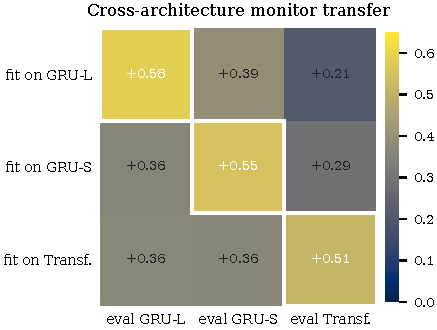
\includegraphics[width=0.85\columnwidth]{figures/architecture_transfer.pdf}
\caption{Cross-architecture monitor transfer (Spearman). Boxed cells are same-architecture
references. Single seed, $K=3$.}
\label{fig:archtransfer}
\end{figure}

\begin{table}[t]
\centering\small
\begin{tabular}{lccc}
\toprule
& eval GRU-L & eval GRU-S & eval Transf. \\
\midrule
fitted on GRU-L & \emph{+0.584} & +0.391 & +0.207 \\
fitted on GRU-S & +0.356 & \emph{+0.551} & +0.288 \\
fitted on Transf. & +0.363 & +0.362 & \emph{+0.513} \\
\bottomrule
\end{tabular}
\caption{Monitor fitted on one architecture, evaluated on another's A-test. Italic entries are
same-architecture references. Single seed, $K=3$.}
\label{tab:archtransfer}
\end{table}

\subsection{Restoration is selective across shift types}
\label{sec:asym}

We pre-registered a two-family account of transfer and tested it predictively on two new
configurations. The geometric half was confirmed: on E, never seen and drawn from a different
maze family, $\mathrm{A{+}B}\to$E reaches $\rho = 0.855$ against a no-exposure baseline of
$0.116$, and E acts as a donor ($\mathrm{A{+}E}\to$D gives $0.800$). The noise-driven half was
not: $\mathrm{A{+}C}\to$F3 reaches $0.444$ against a pre-registered bar of $0.50$.
\textbf{We therefore withdraw the taxonomy} and report only the asymmetry the data support
(Figure~\ref{fig:asym}):
\begin{center}\small
\begin{tabular}{lcc}
\toprule
donor $\downarrow$ / recipient $\rightarrow$ & geometric & noise-driven \\
\midrule
geometric (B, E) & $0.73$--$0.86$ & $\approx 0.31$ \\
noise-driven (C, F3) & $0.39$--$0.54$ & $0.44$--$0.47$ \\
\bottomrule
\end{tabular}
\end{center}
Geometric donors transfer strongly to geometric recipients and weakly to noise-driven ones;
noise donors transfer moderately to everything. \S\ref{sec:mech} gives the mechanism.

Two caveats. The pattern rests on four donors within one environment family. And donors differ
in \emph{severity} as well as in kind, so an account in which transfer depends on how much the
donor degrades the model --- rather than on the type of shift --- is not excluded by these
experiments.

\begin{figure}[t]
\centering
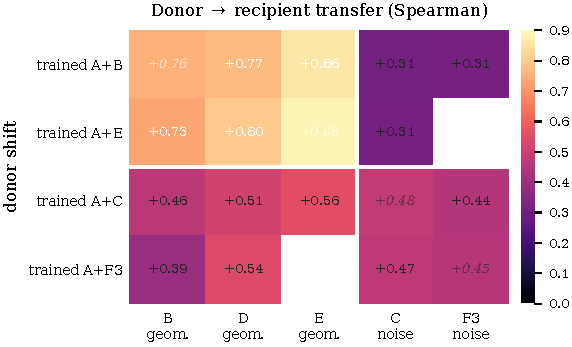
\includegraphics[width=\columnwidth]{figures/shift_asymmetry.pdf}
\caption{Donor--recipient transfer. White lines separate geometric from noise-driven
configurations; italic cells evaluate a donor on itself. The top-right quadrant --- geometric
donors on noise-driven recipients --- is the weakest.}
\label{fig:asym}
\end{figure}

\subsection{A weak test of downstream utility}
\label{sec:planning}

We also tested whether the monitor improves planning by setting the imagination horizon
adaptively in a model-predictive controller. It does not: adaptive planning reached success
$0.517 \pm 0.065$ against $0.933 \pm 0.032$ for the best fixed horizon, at $5.49\times$ the
imagination compute. However, success fell \emph{monotonically} with horizon, so the
compute--performance frontier had no interior optimum and there was nothing for an adaptive
rule to find; our attempt to make the task non-myopic did not take (mean detour $0.13$ cells).
We report this as a \textbf{weak test} rather than a refutation. Details in the appendix.

\section{Mechanistic Analysis}
\label{sec:mech}

Why does the monitor fail under shift, and why do input corrections not help?

Write $\rho_D(u) = \rho\big(u, \Hstar \mid D\big)$ for the within-distribution rank correlation
between a scalar feature $u$ and the horizon on distribution $D$. It is useful to separate two
things a shift can do to a feature:
\begin{align}
\text{scale shift:} \quad & \mathbb{E}_{D'}[u] \ne \mathbb{E}_{D}[u], \quad \rho_{D'}(u) \approx \rho_{D}(u), \\
\text{rank shift:} \quad & |\rho_{D'}(u)| \ll |\rho_{D}(u)|.
\end{align}
A monotone reparameterisation of $u$ --- rank normalisation included --- can absorb a scale
shift. It cannot absorb a rank shift, because it preserves the ordering it is given, and under
a rank shift that ordering has stopped carrying information about $\Hstar$.

The dominant in-distribution feature, the spread of imagined displacement across ensemble
members, undergoes a rank shift. Its mean \emph{rises} from $0.517$ in distribution to
$0.986$, $1.455$ and $0.971$ on B, C and D --- so aggregate separation between distributions is
retained --- while $\rho_D$ collapses from $-0.446$ to $-0.111$, $-0.191$ and $-0.089$. The
signal still reports \emph{that} matters are harder; it stops reporting \emph{which states}
will fail. This is the direct explanation of \S\ref{sec:repair}: rank normalisation is exactly
the operation that cannot help here.

Two further observations. Predictive entropy moves in the \emph{wrong} direction under shift,
its $\rho_D$ going from $-0.394$ in distribution to $+0.001$ on D, whereas ensemble spread
retains its sign. \citet{berger2026biased} report a related but distinct effect: uncertainty
\emph{declining along} an extended latent rollout as it is drawn into well-modelled attractor
regions. We measure across-distribution means and within-distribution rank correlations rather
than the within-rollout trajectory of uncertainty, so our observations neither confirm nor
contradict that account; establishing whether the two mechanisms coincide would require
measuring uncertainty along the rollout, which we did not do. What our data do show is that the
failure is not confined to one signal family: entropy and ensemble spread degrade differently,
and no feature we measured is both stable and useful --- the feature with the lowest rank
instability has $\rho \approx 0$ everywhere (Figure~\ref{fig:featstab}).

That figure also explains the asymmetry of \S\ref{sec:asym}. One feature --- how far the agent
can currently see unobstructed --- is \emph{useless} in distribution ($\rho = +0.004$) and
\emph{dominant} under geometric shift ($+0.586$, $+0.566$, $+0.533$ on B, D, E). A monitor
trained only on A has no reason to use it; exposure to a geometric shift teaches it to. On
noise-driven configurations the same feature is inert ($+0.024$, $-0.015$, $-0.031$). A cue
that rescues geometric shifts therefore cannot rescue noise-driven ones, and we find no
equivalent single carrier on the noise side --- which is why those donors transfer broadly but
never strongly.

\begin{figure}[t]
\centering
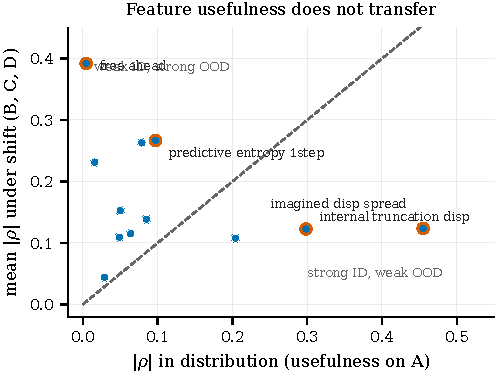
\includegraphics[width=0.92\columnwidth]{figures/feature_stability.pdf}
\caption{In-distribution usefulness against usefulness under shift, per uncertainty feature.
Points far below the diagonal undergo a rank shift; the circled point near the $y$-axis is
useless in distribution yet dominant under geometric shift.}
\label{fig:featstab}
\end{figure}

\section{Limitations}
\label{sec:limits}

\textbf{One environment family.} All experiments use MiniGrid with symbolic observations and
world models of roughly $2.8$M parameters. The mechanism we identify --- a cue that is useless
in distribution and dominant under shift --- is instantiated by a domain-specific feature, and
whether an analogue exists for pixel-based or continuous-control world models is untested.

\textbf{Censoring.} $21\%$ of A-test targets sit at $H_{\max} = 30$. MAE is inflated and the
upper tail of $\Hstar$ is unidentified; a larger $H_{\max}$ would settle this.

\textbf{Effect size.} $R^2 = 0.318$: most variance in $\Hstar$ is unexplained, and the margin
over the optimistic ceiling is about $1$ MAE against a target with s.d.\ $\approx 10.3$ ---
statistically robust, quantitatively modest.

\textbf{Architecture evidence is single-seed.} \S\ref{sec:arch} uses one seed and $K=3$ per
architecture. It establishes that the phenomenon occurs without recurrence; it does not support
comparisons between architectures.

\textbf{Few shift families, and a severity confound.} The asymmetry rests on four donors. Two
configurations (observation noise at $15\%$ and $70\%$) failed a pre-registered validity gate
because they barely degraded the model, leaving two instruments on the noise-driven side. Donor
severity and type covary.

\textbf{Downstream utility untested.} The planning experiment was a weak test
(\S\ref{sec:planning}); we make no claim that the monitor improves control.

\section{Discussion}
\label{sec:discussion}

Our results support a bounded statement: a world model can learn a useful monitor of the
reliability horizon of its imagined futures, but that monitor is distribution-dependent and
only partially transferable across architectures and shift types.

The practical reading is uncomfortable for uncertainty-gated imagination. A monitor fitted where
the model works will be most confident where the model fails, and input-level corrections do not
help, because features stop \emph{ranking} states rather than being mis-scaled. Exposure to
failures does help --- selectively, and less so when the world model is already strong.

This suggests reading reliability monitoring less as reading out an intrinsic property of
uncertainty and more as a learned model of one's own failures, whose validity is inherited from
the distribution of failures encountered during training. The asymmetry sharpens the point: what
a monitor learns from one kind of failure may be a specific cue rather than a general capacity
for caution.

\section{Conclusion}
\label{sec:conclusion}

We defined an operational reliability horizon for imagined rollouts and showed that a learned
monitor predicts it beyond an optimistically fitted monotone single-scalar ceiling, provided it
may inspect the imagined rollout. The monitor fails anti-conservatively under distribution
shift; rank normalisation and novelty gating do not repair it; exposure to an appropriate
shifted distribution substantially restores transfer without being explained by sample count
alone; and that restoration is selective across shift types and does not replicate in a
world model that degrades less. Of nine pre-registered hypotheses, three were supported and
five were not; the negative results carry most of the content.

\section*{Reproducibility}

All thresholds, splits and seeds were frozen before the corresponding evaluations in five
pre-registration documents, with departures logged, and every number here is emitted
programmatically from stored artifacts. Code, pre-registration protocols, the deviation ledger
and per-seed statistics are available at \url{https://github.com/abhishekrajdhar/reliability_in_worldmodel}; the appendix documents architectures,
hyperparameters, features, statistics, censoring and the rejected instruments.

\bibliographystyle{plainnat}
\bibliography{references}

\end{document}
